%
% HR.tex
% Human Resources
%
% Aleph Objects Operations Manual
%
% Copyright (C) 2014, 2015 Aleph Objects, Inc.
%
% This document is licensed under the Creative Commons Attribution 4.0
% International Public License (CC BY-SA 4.0) by Aleph Objects, Inc.
%

\section{Professional Employment Organizations (PEO)}
Insperity.

\section{Employee Benefits}
See employee handbook at \texttt{http://esc.insperitiy.com}

\section{Logging hours in OpenERP}
For hourly Insperity employees:

OpenERP ---> Human Resources ---> Attendences ---> Attendences

For hourly Kelly employees, track your hours on Kelly's website.

\section{Requesting time off in OpenERP}
OpenERP ---> Human Resources ---> Leaves ---> Leave Requests

\section{Recruitment / Interviewing}
Kelly, Insperity, JobZology.

\section{Performance}
Insperity.

\section{Training}
Certifications.

\section{Organizational Chart}
See figure \ref{fig:ao_org_chart} for Aleph Object's organizational chart.
%
% OrgChart.tex
% HR Organizational Chart
%
% Aleph Objects Operations Manual
%
% Copyright (C) 2014, 2015 Aleph Objects, Inc.
%
% This document is licensed under the Creative Commons Attribution 4.0
% International Public License (CC BY-SA 4.0) by Aleph Objects, Inc.

\begin{sidewaysfigure}[p]
\thisfloatpagestyle{empty}
\begin{center}
\resizebox{\textwidth}{!}
{
\begin{forest}
for tree={
  draw,
  minimum height=3cm,
  anchor=north,
  align=center,
  child anchor=north,
  inner sep=5mm,
  s sep=5mm
},
[{CEO}, align=center, for tree={rectangle}, fill=ao-purple, tier=first
    [{CTO}, for tree={fill=pink}, tier=second, child anchor=east
        [{Engineer\\Assistant}, tier=third
            [{Cluster\\Tech}, tier=fourth]
            [{Cluster\\Tech}, tier=fourth]
        ]
        [{Engineer\\Assistant}, tier=third]
      [{VP Mfg}, for tree={fill=ao-light-orange}, tier=third
            [{Assembly\\Lead}, for tree={fill=ao-light-orange}, tier=fourth
                [{Assembly\\I}, tier=fifth]
                [{Assembly\\I}, tier=fifth]
                [{Assembly\\II}, tier=fifth]
                [{Assembly\\II}, tier=fifth]
                [{Assembly\\II}, tier=fifth]
                [{Assembly\\II}, tier=fifth]
            ]
        ]
    ]
    [{Bookkeeper}, fill=ao-gold], tier=second
    [{SysAdmin}, fill=ao-dark-blue], tier=second
    [{COO}, for tree={fill=ao-light-blue}, tier=second child anchor=west
        [{Shipping\\Manager}, tier=third]
        [{Sales\\Manager}, tier=third]
        [{Programmer}, tier=third]
        [{Comms}, tier=third]
        [{CSR}, tier=third]
    ]
]
\end{forest}
}
\end{center}
\caption{Organizational Chart}
 \label{fig:ao_org_chart}
\end{sidewaysfigure}


See figure \ref{fig:ao_org_chart_dot} for Aleph Object's organizational chart in dot.

\begin{sidewaysfigure}[p]
\thisfloatpagestyle{empty}
% The ao-orgchart-dot.png was built in dot.
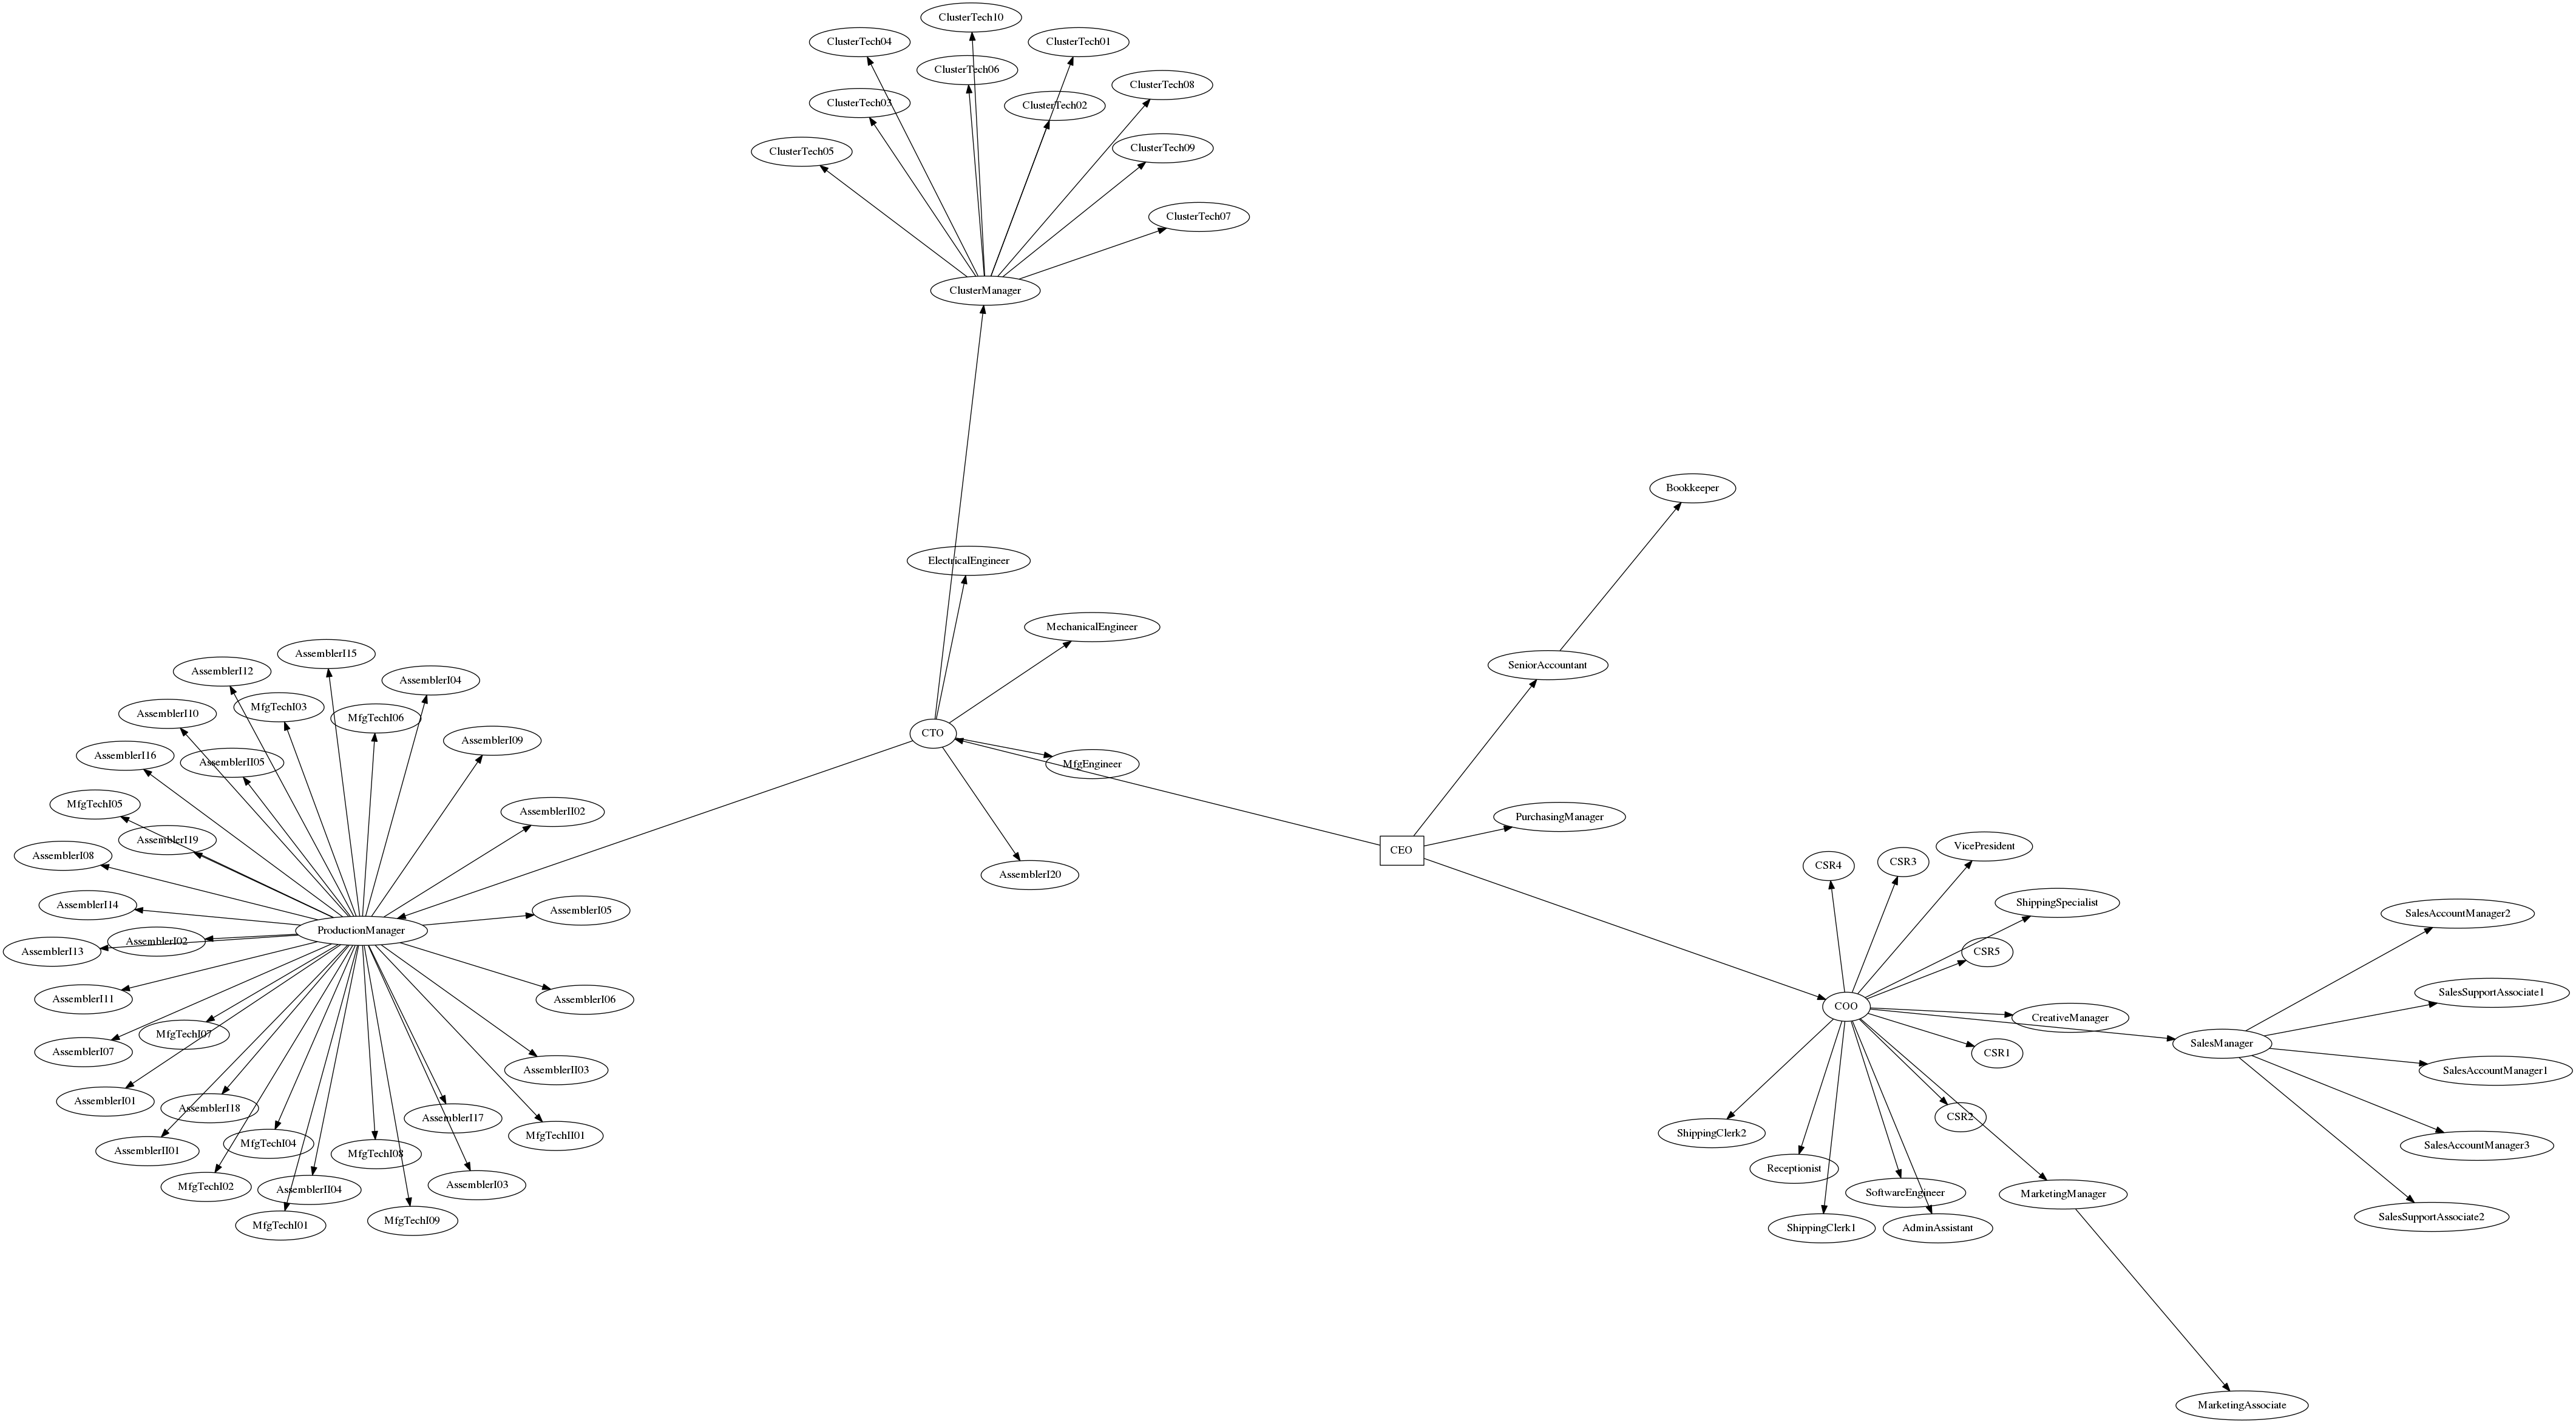
\includegraphics[keepaspectratio=true,height=1.10\textheight,width=1.00\textwidth,angle=]{ao-orgchart-dot.png}
 \caption{Aleph Objects Org Chart dot}
 \label{fig:ao_org_chart_dot}
\end{sidewaysfigure}

\section{Schedules}
The following calendars list when there are recurring meetings.

%
% SchedWeek.tex
% Weekly Recurring Events Schedule
%
% Aleph Objects Operations Manual
%
% Copyright (C) 2014 Aleph Objects, Inc.
%
% This document is licensed under the Creative Commons Attribution 4.0
% International Public License (CC BY-SA 4.0) by Aleph Objects, Inc.
%

% To extract just the schedule pages from the PDF, run something like:
% pdfjoin AOOM.pdf 31-32 -o AOOM-schedule.pdf

% These set the width of a day and the height of an hour.
\newcommand*\daywidth{3.7cm}
\newcommand*\hourheight{3.8em}

% The entry style will have two options:
% * the first option sets how many hours the entry will be (i.e. its height);
% * the second option sets how many overlapping entries there are (thus
%   determining the width).
\tikzset{entry/.style 2 args={
    xshift=(0.5334em+0.8pt)/2,
    draw,
    line width=0.8pt,
    font=\sffamily,
    rectangle,
    rounded corners,
    fill=blue!20,
    anchor=north west,
    inner sep=0.3333em,
    text width={\daywidth/#2-1.2em-1.6pt},
    minimum height=#1*\hourheight,
    align=center
}}

% Start the picture and set the x coordinate to correspond to days and the y
% coordinate to correspond to hours (y should point downwards).
\begin{sidewaysfigure}[p]
\thisfloatpagestyle{empty}
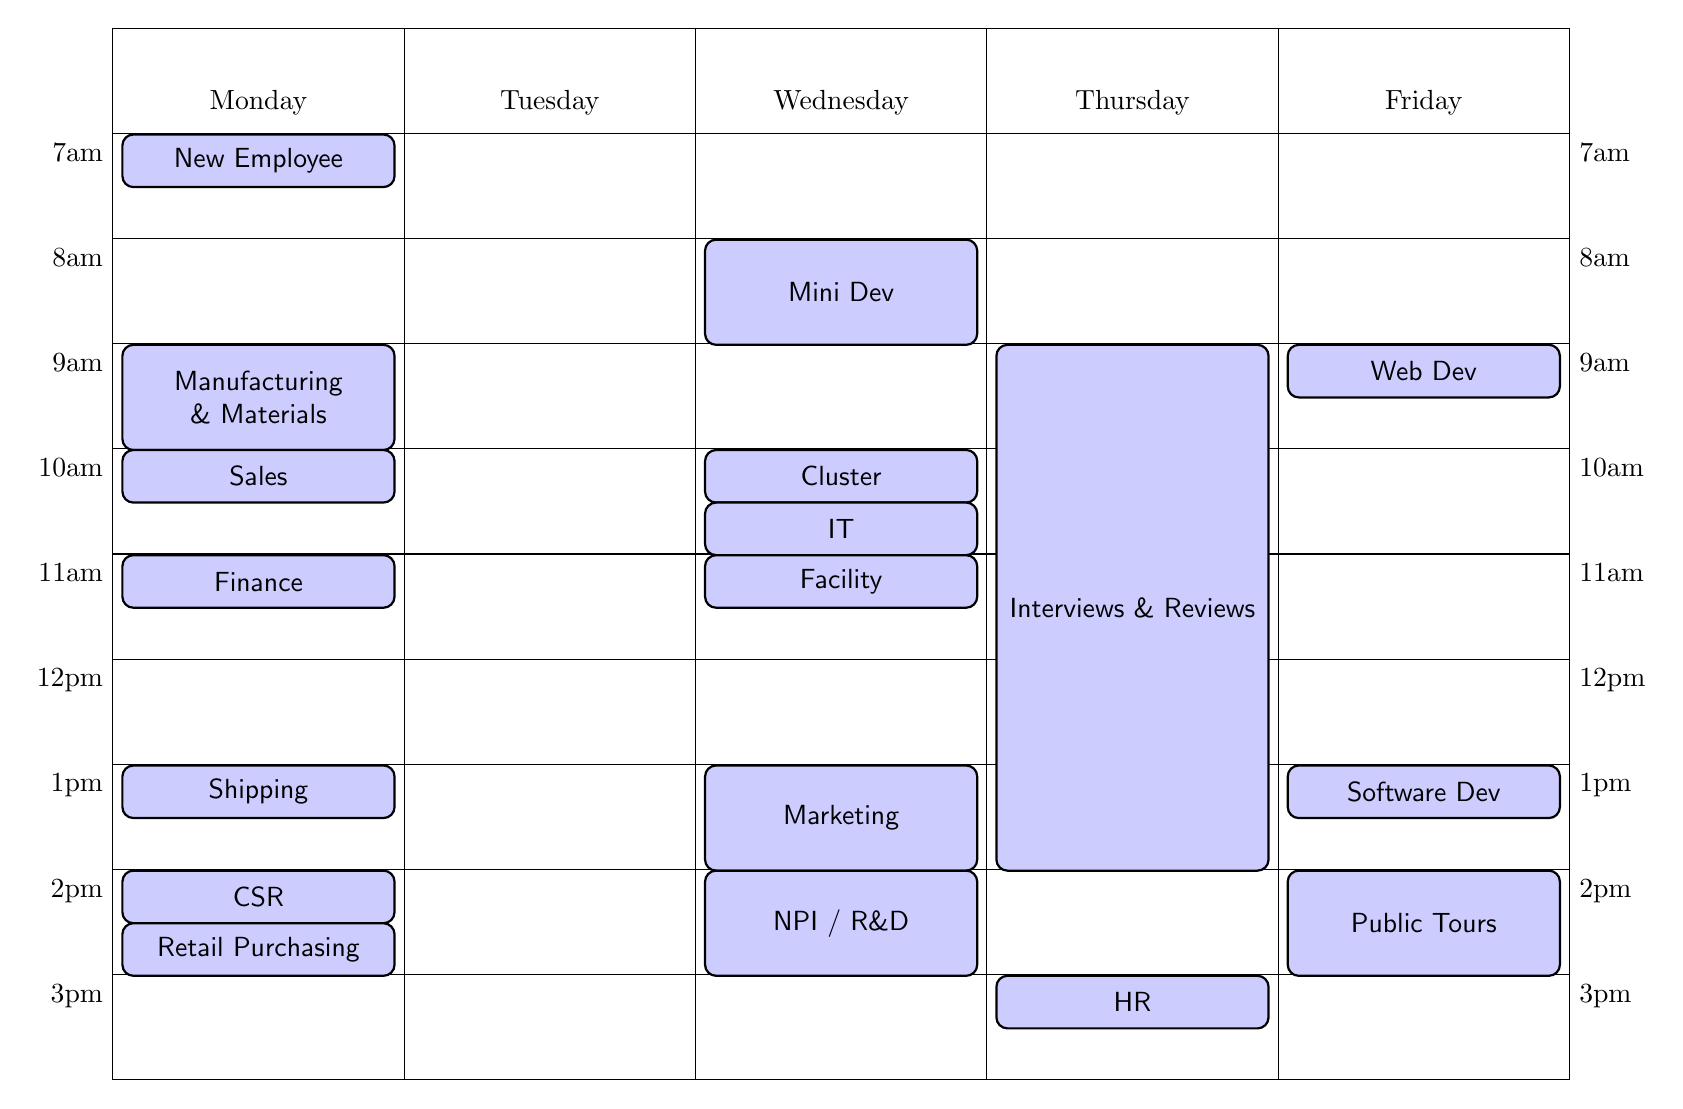
\begin{tikzpicture}[y=-\hourheight,x=\daywidth]

    % First print a list of times.
    \foreach \time/\ustime in {7/7am,8/8am,9/9am,10/10am,11/11am,12/12pm,13/1pm,14/2pm,15/3pm}
        \node[anchor=north east] at (1,\time) {\ustime};

    % Draw some day dividers.
    \draw (1,6) -- (1,16);
    \draw (2,6) -- (2,16);
    \draw (3,6) -- (3,16);
    \draw (4,6) -- (4,16);
    \draw (5,6) -- (5,16);
    \draw (6,6) -- (6,16);
    
    % Draw some hour dividers.
    \draw (1,6) -- (6,6);
    \draw (1,7) -- (6,7);
    \draw (1,8) -- (6,8);
    \draw (1,9) -- (6,9);
    \draw (1,10) -- (6,10);
    \draw (1,11) -- (6,11);
    \draw (1,12) -- (6,12);
    \draw (1,13) -- (6,13);
    \draw (1,14) -- (6,14);
    \draw (1,15) -- (6,15);
    \draw (1,16) -- (6,16);

    \foreach \time/\ustime in {7/7am,8/8am,9/9am,10/10am,11/11am,12/12pm,13/1pm,14/2pm,15/3pm}
        \node[anchor=north west] at (6,\time) {\ustime};
        
    % Start Monday.
    % Write the entries. Note that the x coordinate is 1 (for Monday) plus an
    % appropriate amount of shifting. The y coordinate is simply the starting
    % time.
    % 1=Monday, 2=Tuesday, 3=Wednesday, 4=Thursday, 5=Friday
    %\node[entry={DURATION}{COLUMN WIDTH?}] at (DAY,HOUR) {TEXT};
    \node[anchor=north] at (1.5,6.5) {Monday};
    \node[entry={0.5}{1}] at (1,7) {New Employee};
    \node[entry={1.0}{1}] at (1,9) {Manufacturing \& Materials};
    \node[entry={0.5}{1}] at (1,10){Sales};
    \node[entry={0.5}{1}] at (1,11) {Finance};
    \node[entry={0.5}{1}] at (1,13) {Shipping};
    \node[entry={0.5}{1}] at (1,14) {CSR};
    \node[entry={0.5}{1}] at (1,14.5) {Retail Purchasing};

    % Tuesday
    \node[anchor=north] at (2.5,6.5) {Tuesday};
    
    % Wednesday
    \node[anchor=north] at (3.5,6.5) {Wednesday};
    \node[entry={1.0}{1}] at (3,8) {Mini Dev};
    \node[entry={0.5}{1}] at (3,10) {Cluster};
    \node[entry={0.5}{1}] at (3,10.5) {IT};
    \node[entry={0.5}{1}] at (3,11) {Facility};
    \node[entry={1.0}{1}] at (3,13) {Marketing};
    \node[entry={1.0}{1}] at (3,14) {NPI / R\&D};
    
    % Thursday
    \node[anchor=north] at (4.5,6.5) {Thursday};
    \node[entry={5.0}{1}] at (4,9) {Interviews \& Reviews};
    \node[entry={0.5}{1}] at (4,15) {HR};
    
    % Friday
    \node[anchor=north] at (5.5,6.5) {Friday};
    \node[entry={0.5}{1}] at (5,9) {Web Dev};
    \node[entry={0.5}{1}] at (5,13) {Software Dev};
    \node[entry={1.0}{1}] at (5,14) {Public Tours};

\end{tikzpicture}
\caption{Weekly Company Meetings}
 \label{fig:ao_week_meet}
\end{sidewaysfigure}


See figure \ref{fig:ao_week_meet} for Aleph Object's weekly meeting schedule.
%
% SchedMonth.tex
% Recurring Events Schedule
%
% Aleph Objects Operations Manual
%
% Copyright (C) 2014, 2015 Aleph Objects, Inc.
%
% This document is licensed under the Creative Commons Attribution 4.0
% International Public License (CC BY-SA 4.0) by Aleph Objects, Inc.
%

%%% Monthly Meeting
\newcommand{\calrow}[1]{%
%\node[anchor=base,xshift=0.5ex](sun){S};
%\node[base right=of sun](mon){M};
\node[anchor=base,xshift=0.5ex](mon){M};
\node[base right=of mon](tue){T};
\node[base right=of tue](wed){W};
\node[base right=of wed](thu){T};
%\node[base right=of thu](fri){\ \!F};
%\node[base right=of fri](sat){\ \!S};
\node[base right=of thu](fri){F};
\node[base right=of fri](sat){S};
\node[base right=of sat](sun){S};
\node[black,above=of thu]{\textbf{#1}};
}

\newcommand{\calperiod}[1]{\calendar[dates=\the\year-#1-01 to \the\year-#1-last,
  every day/.style={anchor=base}, % Center days
  day text={\%d=},rounded corners=0,anchor=base,text height=1ex,text depth=-0.5ex]
\holidays;}

% Company Holidays 2015:
% New Year's Day 2015-01-01 - Thursday
% Memorial Day 2015-05-25 - Monday
% Independence Day 2015-07-04 - Saturday
% Labor Day - 2015-09-07 - Monday
% Thanksgiving Day - 2015-11-26 - Thursday
% Day after Thanksgiving - 2015-11-27 - Friday
% Christmas - 2015-12-25 - Friday

% Company meetings, the first business day of the month at 8AM, for 2015.
\newcommand{\holidays}{
if (equals=01-02) {\node [fill=yellow,draw,star] {};}
if (equals=02-02) {\node [fill=yellow,draw,star] {};}
if (equals=03-02) {\node [fill=yellow,draw,star] {};}
if (equals=04-01) {\node [fill=yellow,draw,star] {};}
if (equals=05-01) {\node [fill=yellow,draw,star] {};}
if (equals=06-01) {\node [fill=yellow,draw,star] {};}
if (equals=07-01) {\node [fill=yellow,draw,star] {};}
if (equals=08-03) {\node [fill=yellow,draw,star] {};}
if (equals=09-01) {\node [fill=yellow,draw,star] {};}
if (equals=10-01) {\node [fill=yellow,draw,star] {};}
if (equals=11-02) {\node [fill=yellow,draw,star] {};}
if (equals=12-01) {\node [fill=yellow,draw,star] {};}
}

\begin{figure}
\thisfloatpagestyle{empty}
\begin{tikzpicture}
[every calendar/.style={week list}]
\sffamily
\matrix[%
row 1/.style={black,node distance=.3ex},%
row 3/.style={black,node distance=.3ex},%
row 5/.style={black,node distance=.3ex},%
row 7/.style={black,node distance=.3ex},
column sep=1ex,%
draw=black,thick,rounded corners=30pt,%
postaction={decorate,decoration={markings,mark=at position 0.51 with
{\node[fill=white,text=black,font={\bfseries\Large}] (year) {\the\year};}}}
]{%
\calrow{January} & \calrow{February} & \calrow{March} \\
\calperiod{01} & \calperiod{02} & \calperiod{03} \\[0.4cm]
\calrow{April} & \calrow{May} & \calrow{June} \\
\calperiod{04} & \calperiod{05} & \calperiod{06} \\[0.4cm]
\calrow{July} & \calrow{August} & \calrow{September} \\
\calperiod{07} & \calperiod{08} & \calperiod{09} \\[0.4cm]
\calrow{October} & \calrow{November} & \calrow{December} \\
\calperiod{10} & \calperiod{11} & \calperiod{12} \\[0.4cm]
};
\end{tikzpicture}
\caption{Monthly Company Meetings at 8:00AM MST}
 \label{fig:ao_month_meet}
\end{figure}

See figure \ref{fig:ao_month_meet} for Aleph Object's monthly company meeting schedule.
